\section{Algorytm kNN}
\label{chap:knn}
Algorytm kNN (ang. \textit{k Nearest Neighbours})  jest jednym z najprostszych algorytmów klasyfikacyjnych, należy również do najpopularniejszych ze względu na prostotę implementacji oraz dobre wyniki obliczeń. Reguła klasyfikacji opiera się na założeniu, że dane przedstawione w $n$-wymiarowej przestrzeni zgrupowane będą w obszarach opisanych podobnymi cechami. Bazując na tym założeniu, ustalenie klasy dla wektora wejściowego sprowadza się do zbadania jego najbliższego otoczenia w przestrzeni i wyboru klasy najczęściej w nim występującej.

Pierwszym krokiem algorytmu jest wyznaczenie odległości pomiędzy próbką ze zbioru testowego, oraz wszystkimi próbkami ze zbioru uczącego. Najczęściej stosowaną metodą wyznaczania odległości jest metryka euklidesowa dana poniższym wzorem, gdzie $N$ to szerokość wektora dla każdej próbki:

\begin{equation}
d(x,y) = \sum_{i=1}^{N} \sqrt{(x_i - y_i)^2}.
\end{equation}

Następnie ze zbioru $K$ najbliższych sąsiadów wybierana jest najczęściej występująca klasa obiektów, a rozważany przypadek klasyfikowany jest jako obiekt tej klasy. Dobór optymalnego parametru $K$ odbywa się zazwyczaj na drodze eksperymentów stosując nieparzyste wartości $K=1,3,5...$ . Proces uczenia jest bardzo prosty i ogranicza się do zapamiętania wszystkich próbek ze zbioru uczącego. Konieczność wyznaczenia odległości pomiędzy klasyfikowaną próbką a wszystkimi próbkami ze zbioru uczącego wymusza rozważne przygotowanie tego ostatniego. Zawarte w nim wartości powinny dobrze definiować całą przestrzeń, jednocześnie minimalizując rozmiar w celu przyspieszenia działania algorytmu. Poza klasyfikacją algorytm kNN wykorzystywany jest także do klasteryzacji, regresji, estymowania funkcji gęstości. W 2006 roku algorytm został zaliczony do 10 najpopularniejszych algorytmów w dziedzinie eksploracji danych podczas konferencji IEEE w Hong Kongu.

Zasadę działania algorytmu na przykładzie przedstawiono na rysunku \ref{fig:knn-idea}.

\begin{figure}[H]
	\centering
	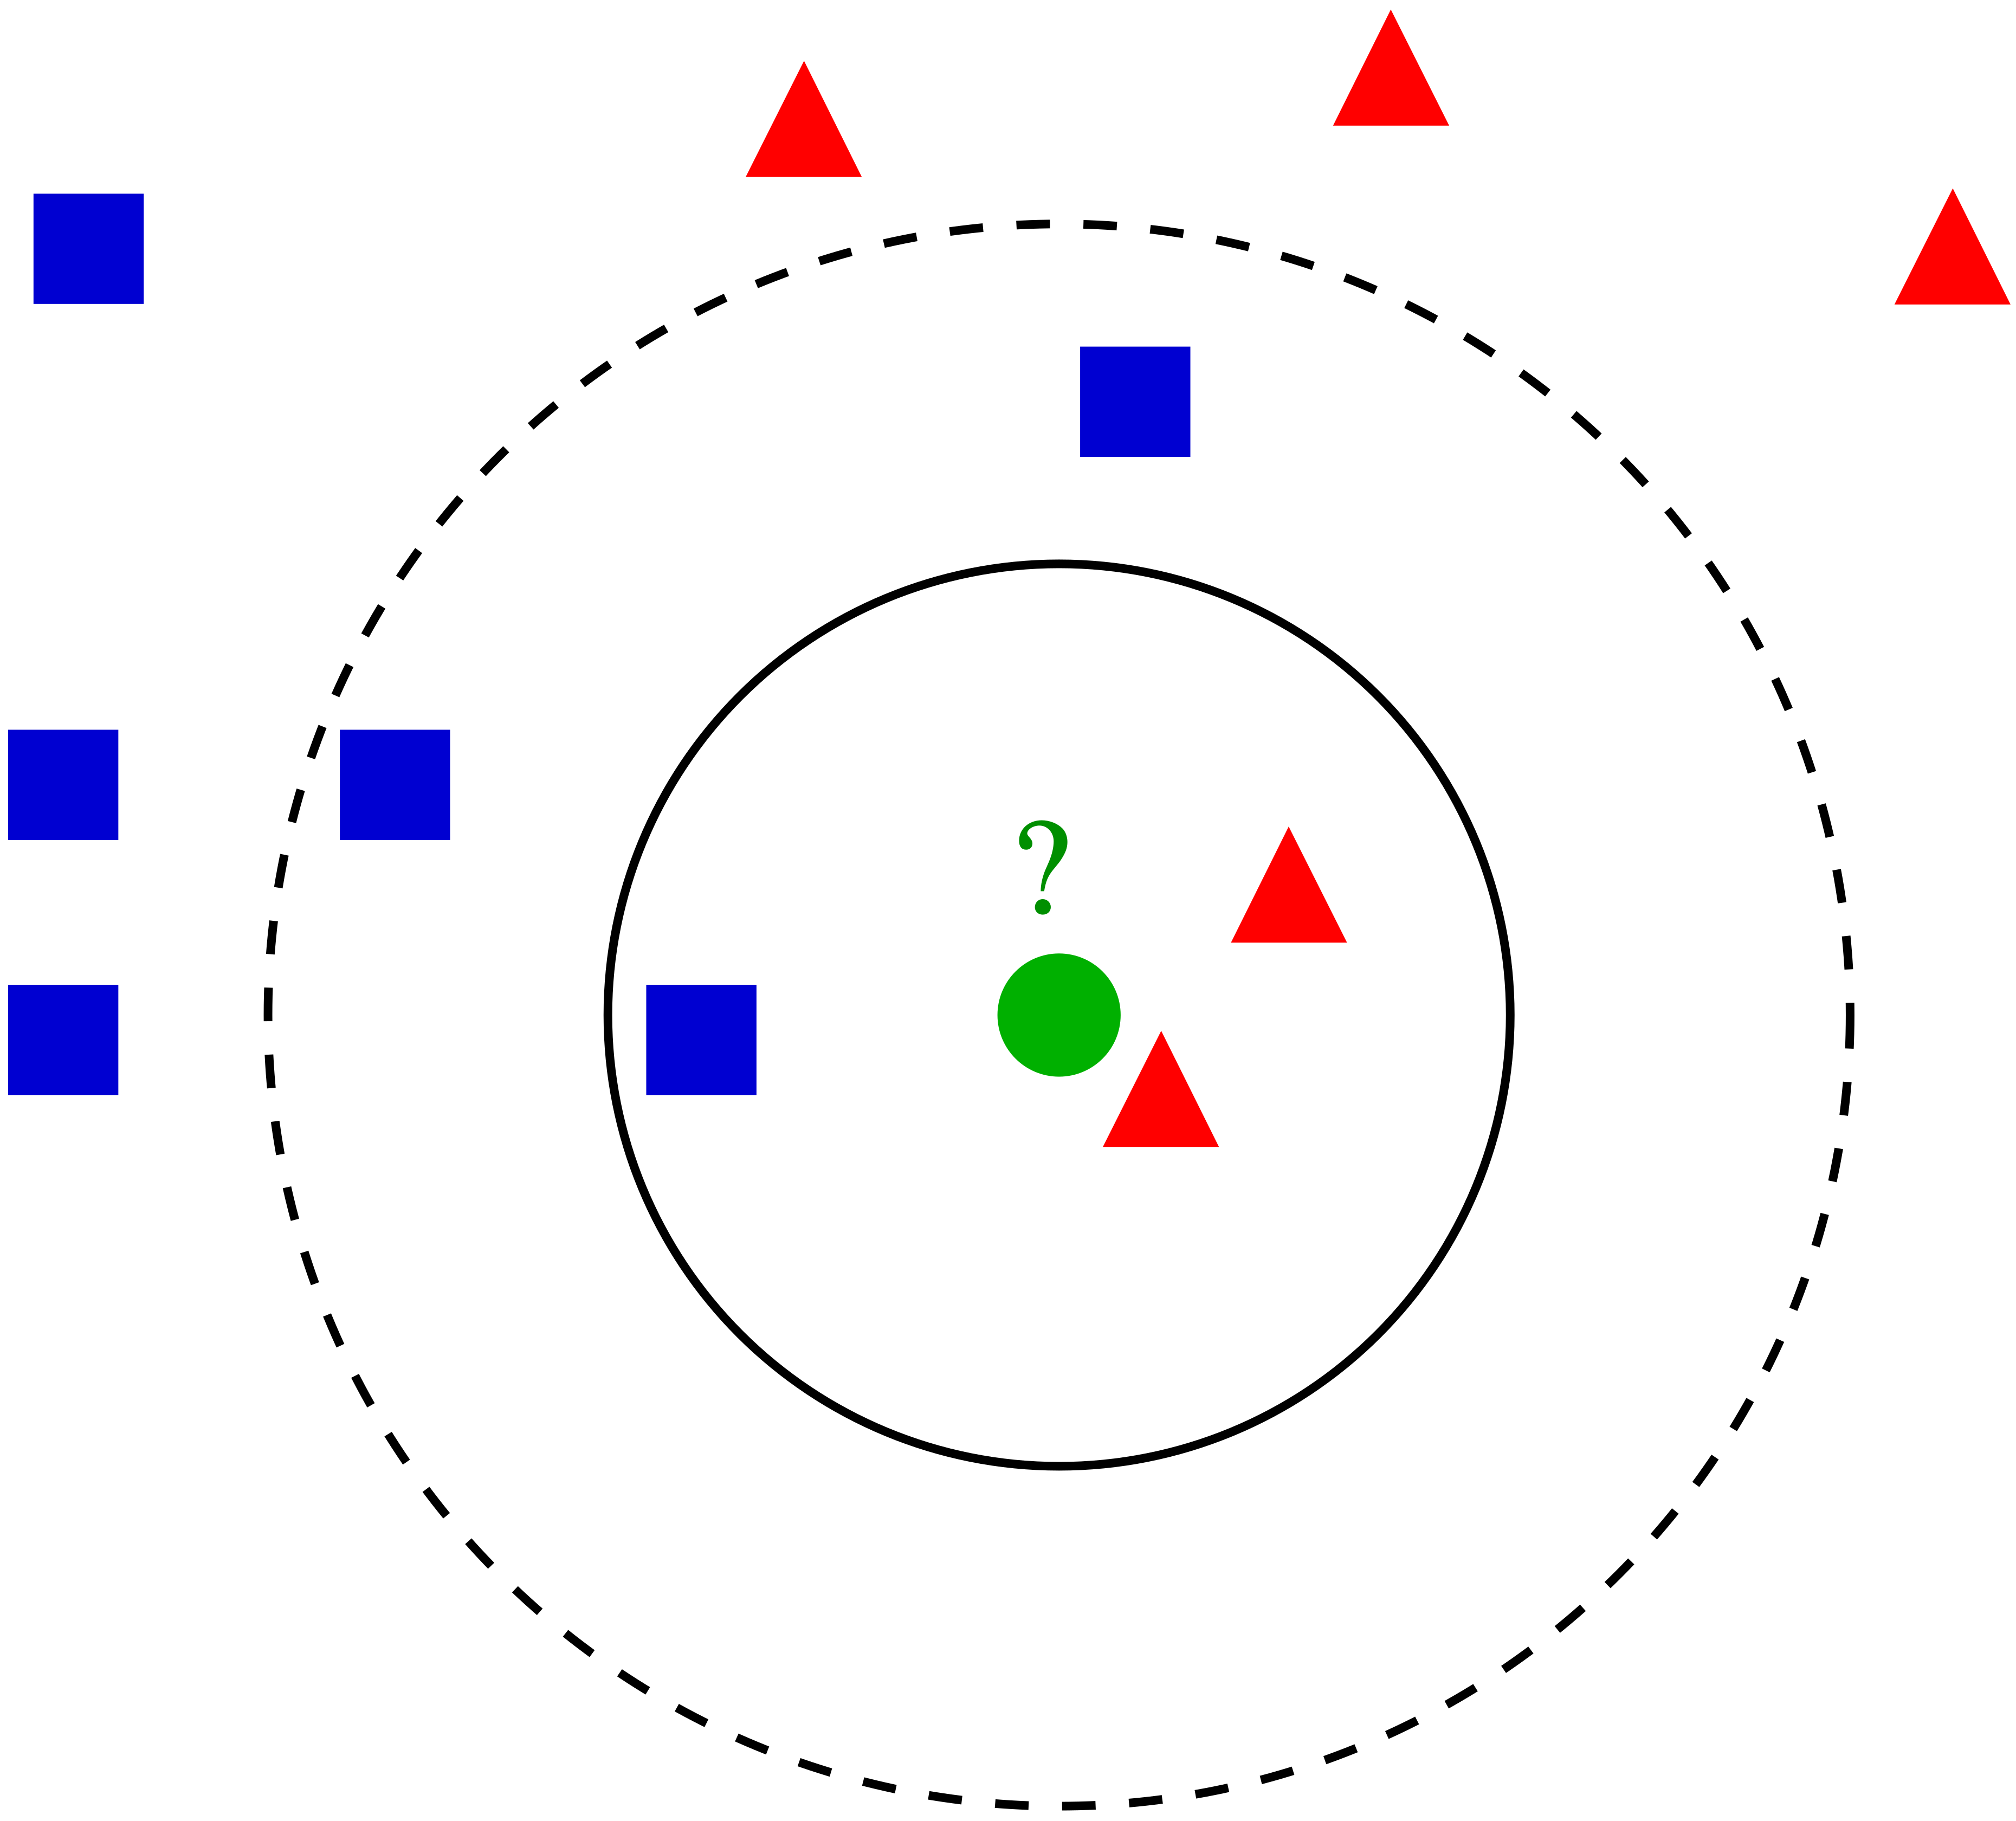
\includegraphics[width=10cm]{img/KnnClassification}
	\caption{Schematyczne przedstawienie klasyfikacji dwuwymiarowego wektora danych. Źródło \cite{knn-wiki}}
	\label{fig:knn-idea}
\end{figure}

Zadaniem klasyfikacji jest ustalenie przynależności wartości wejściowej - koła, do jednej z dwóch grup elementów - kwadratów i trójkątów. Przyjmując wartość parametru $K=3$ (linia ciągła na rysunku), wartość przypisana zostanie do grupy zawierającej trójkąty. Zakładając $K=5$ wynik będzie przeciwny i element zostanie powiązany z grupą zawierającą kwadraty.

Dobór wartości parametru $K$ dającej najlepsze wyniki wymaga więc znajomości badanego zjawiska bądź przeprowadzenia doświadczeń na reprezentatywnym zbiorze testowym.
